%% For double-blind review submission, w/o CCS and ACM Reference (max submission space)
\documentclass[sigplan]{acmart}\settopmatter{printfolios=true,printccs=false,printacmref=false}
%% For double-blind review submission, w/ CCS and ACM Reference
%\documentclass[sigplan,review,anonymous]{acmart}\settopmatter{printfolios=true}
%% For single-blind review submission, w/o CCS and ACM Reference (max submission space)
%\documentclass[sigplan,review]{acmart}\settopmatter{printfolios=true,printccs=false,printacmref=false}
%% For single-blind review submission, w/ CCS and ACM Reference
%\documentclass[sigplan,review]{acmart}\settopmatter{printfolios=true}
%% For final camera-ready submission, w/ required CCS and ACM Reference
%\documentclass[sigplan]{acmart}\settopmatter{}


%% Conference information
%% Supplied to authors by publisher for camera-ready submission;
%% use defaults for review submission.
\acmConference[PL'18]{ACM SIGPLAN Conference on Programming Languages}{January 01--03, 2018}{New York, NY, USA}
\acmYear{2018}
\acmISBN{} % \acmISBN{978-x-xxxx-xxxx-x/YY/MM}
\acmDOI{} % \acmDOI{10.1145/nnnnnnn.nnnnnnn}
\startPage{1}

%% Copyright information
%% Supplied to authors (based on authors' rights management selection;
%% see authors.acm.org) by publisher for camera-ready submission;
%% use 'none' for review submission.
\setcopyright{none}
%\setcopyright{acmcopyright}
%\setcopyright{acmlicensed}
%\setcopyright{rightsretained}
%\copyrightyear{2018}           %% If different from \acmYear

%% Bibliography style
\bibliographystyle{ACM-Reference-Format}
%% Citation style
%\citestyle{acmauthoryear}  %% For author/year citations
%\citestyle{acmnumeric}     %% For numeric citations
%\setcitestyle{nosort}      %% With 'acmnumeric', to disable automatic
                            %% sorting of references within a single citation;
                            %% e.g., \cite{Smith99,Carpenter05,Baker12}
                            %% rendered as [14,5,2] rather than [2,5,14].
%\setcitesyle{nocompress}   %% With 'acmnumeric', to disable automatic
                            %% compression of sequential references within a
                            %% single citation;
                            %% e.g., \cite{Baker12,Baker14,Baker16}
                            %% rendered as [2,3,4] rather than [2-4].


%%%%%%%%%%%%%%%%%%%%%%%%%%%%%%%%%%%%%%%%%%%%%%%%%%%%%%%%%%%%%%%%%%%%%%
%% Note: Authors migrating a paper from traditional SIGPLAN
%% proceedings format to PACMPL format must update the
%% '\documentclass' and topmatter commands above; see
%% 'acmart-pacmpl-template.tex'.
%%%%%%%%%%%%%%%%%%%%%%%%%%%%%%%%%%%%%%%%%%%%%%%%%%%%%%%%%%%%%%%%%%%%%%


%% Some recommended packages.
\usepackage{booktabs}   %% For formal tables:
                        %% http://ctan.org/pkg/booktabs
\usepackage{subcaption} %% For complex figures with subfigures/subcaptions
                        %% http://ctan.org/pkg/subcaption

\usepackage{tikz}
\usetikzlibrary{arrows,automata}
\usepackage{tikz-qtree} % Used for syntax trees
\usepackage{tikz-cd} % Used for commutative diagrams

\usepackage{syntax}

\usepackage{semantic}

\usepackage{marginnote}

\usepackage{listings}
\lstset{
  basicstyle=\ttfamily,
  basewidth={.5em,.5em},
}
\newcommand{\ocaml}{\lstinline[language={[objective]caml}]}

%% symbol definitions used throughout the paper

\newcommand{\NT}{\mathbb{N}} % Set of nonterminals
\newcommand{\T}{\mathbb{T}} % Set of terminals
\newcommand{\I}{\mathbb{I}} % Set of identifiers
\newcommand{\yield}{\mathit{yield}} % yield of a parse tree
\newcommand{\semantic}{\mathit{semantic}} % remove semantically unimportant productions from a w' \in L(G')
\newcommand{\parse}{\mathit{parse}} % go from a w' \in L(G') to a subset of L(T)

\begin{document}

%% Title information
\title{Resolvable Ambiguity}         %% [Short Title] is optional;
                                        %% when present, will be used in
                                        %% header instead of Full Title.


%% Author information
%% Contents and number of authors suppressed with 'anonymous'.
%% Each author should be introduced by \author, followed by
%% \authornote (optional), \orcid (optional), \affiliation, and
%% \email.
%% An author may have multiple affiliations and/or emails; repeat the
%% appropriate command.
%% Many elements are not rendered, but should be provided for metadata
%% extraction tools.

%% Author with single affiliation.
\author{Viktor Palmkvist}
\authornote{with author1 note}          %% \authornote is optional;
                                        %% can be repeated if necessary
\orcid{nnnn-nnnn-nnnn-nnnn}             %% \orcid is optional
\affiliation{
  \position{Position1}
  \department{Department1}              %% \department is recommended
  \institution{KTH Royal Institute of Technology}            %% \institution is required
  \streetaddress{Street1 Address1}
  \city{Stockholm}
  \state{State1}
  \postcode{Post-Code1}
  \country{Sweden}                    %% \country is recommended
}
\email{vipa@kth.se}          %% \email is recommended

%% Author with two affiliations and emails.
\author{First2 Last2}
\authornote{with author2 note}          %% \authornote is optional;
                                        %% can be repeated if necessary
\orcid{nnnn-nnnn-nnnn-nnnn}             %% \orcid is optional
\affiliation{
  \position{Position2a}
  \department{Department2a}             %% \department is recommended
  \institution{Institution2a}           %% \institution is required
  \streetaddress{Street2a Address2a}
  \city{City2a}
  \state{State2a}
  \postcode{Post-Code2a}
  \country{Country2a}                   %% \country is recommended
}
\email{first2.last2@inst2a.com}         %% \email is recommended
\affiliation{
  \position{Position2b}
  \department{Department2b}             %% \department is recommended
  \institution{Institution2b}           %% \institution is required
  \streetaddress{Street3b Address2b}
  \city{City2b}
  \state{State2b}
  \postcode{Post-Code2b}
  \country{Country2b}                   %% \country is recommended
}
\email{first2.last2@inst2b.org}         %% \email is recommended


%% Abstract
%% Note: \begin{abstract}...\end{abstract} environment must come
%% before \maketitle command
\begin{abstract}
Text of abstract \ldots.
\end{abstract}


%% 2012 ACM Computing Classification System (CSS) concepts
%% Generate at 'http://dl.acm.org/ccs/ccs.cfm'.
\begin{CCSXML}
<ccs2012>
<concept>
<concept_id>10011007.10011006.10011008</concept_id>
<concept_desc>Software and its engineering~General programming languages</concept_desc>
<concept_significance>500</concept_significance>
</concept>
<concept>
<concept_id>10003456.10003457.10003521.10003525</concept_id>
<concept_desc>Social and professional topics~History of programming languages</concept_desc>
<concept_significance>300</concept_significance>
</concept>
</ccs2012>
\end{CCSXML}

\ccsdesc[500]{Software and its engineering~General programming languages}
\ccsdesc[300]{Social and professional topics~History of programming languages}
%% End of generated code


%% Keywords
%% comma separated list
\keywords{keyword1, keyword2, keyword3}  %% \keywords are mandatory in final camera-ready submission


%% \maketitle
%% Note: \maketitle command must come after title commands, author
%% commands, abstract environment, Computing Classification System
%% environment and commands, and keywords command.
\maketitle


\section{Introduction}

Text of paper \ldots

\subsection{Motivating Ambiguity in Programming Languages}

% TODO: reference PADL paper for this example
Consider the following nested match expression in OCaml:

\begin{lstlisting}[language={[objective]caml}]
match 1 with
  | 1 -> match "one" with
         | str -> str
  | 2 -> "two"
\end{lstlisting}

\noindent The OCaml compiler, when presented with this code, will give a type error for the last line:

\begin{lstlisting}
Error: This pattern matches values of type int
       but a pattern was expected which matches
       values of type string
\end{lstlisting}

\noindent The compiler sees the last line as belonging to the inner \ocaml{match} rather than the outer, as was intended. The fix is simple; put parentheses around the inner match:

\begin{lstlisting}[language={[objective]caml}]
match 1 with
  | 1 -> (match "one" with
          | str -> str)
  | 2 -> "two"
\end{lstlisting}

\noindent The connection between the error message and the fix is not a clear one however; adding parentheses around an expression does not change the type of anything.

To come up with an alternative error to present in this case we look to the OCaml manual for inspiration. It contains an informal description of the syntax of the language\footnote{\url{https://caml.inria.fr/pub/docs/manual-ocaml/language.html}}, in the form of an EBNF-like grammar. Below is an excerpt of the productions for expressions, written in a more standard variant of EBNF:

\setlength{\grammarindent}{5em}
\begin{grammar}
<expr> ::= 'match' <expr> 'with' <pattern-matching>

<pattern-matching> ::= ('|' <pattern> '->' <expr>)+
\end{grammar}

Note that \synt{pattern-matching} is slightly simplified, the original grammar supports \ocaml{when} guards and makes the first \lit{|} optional. If we use this grammar to parse the nested match we find an ambiguity: the last match arm can belong to either the inner match or the outer match. The OCaml compiler makes an arbitrary choice to remove the ambiguity, which may or may not be the alternative the user intended.

We instead argue that the grammar should be left ambiguous for this sort of corner cases that are likely to trip a user, allowing the compiler to present an ambiguity error, which lets the user select the intended alternative.

\subsection{Unresolvable Ambiguity}

Unfortunately, not all ambiguities can be resolved by adding parentheses. Again, looking to the informal OCaml grammar:

\setlength{\grammarindent}{5em}
\begin{grammar}
<expr> ::= <expr> ';' <expr>
  \alt '[' <expr> (';' <expr>)* ';'? ']'
  \alt <constant>
\end{grammar}

\noindent The first production is sequential composition, the second is lists (the empty list is under \synt{constant}). Now consider the following expression: ''\ocaml{[1; 2]}''.

We find that it is ambiguous with two alternatives:
\begin{enumerate}
  \item A list with two elements.
  \item A list with one element, namely a sequential composition.
\end{enumerate}

We can select the second option by putting parentheses around ''\ocaml{1; 2}'', but there is no way to select the first. If the user intended the first option we have a problem: we can present an accurate error message, but there is no way for an end-user to solve it; it requires changes to the grammar itself.

% TODO: ref for undecidable ambiguity checking
To prevent the possibility of an end-user encountering such an error we must ensure that the grammar cannot give rise to an unresolvable ambiguity. It is worth mentioning here that statically checking if a context-free grammar is ambiguous has long been known to be undecidable. Unresolvable ambiguity, however, turns out to be decidable\footnote{With some caveats, I'll talk more about this during the meeting.}.

Note that, as for ambiguity, the shape of the grammar is important, since the property considers parse trees rather than merely words. For this paper, we consider context-free grammars with EBNF operators.

\subsection{Contributions}

\begin{itemize}
  \item Building on \cite{palmkvistCreatingDomainSpecificLanguages2019}, which merely isolates ambiguities, an algorithm that suggests solutions to ambiguity errors.
  \item A formalization of the unresolvable ambiguity property for context-free EBNF grammars.
  \item An algorithm for deciding if a grammar is unresolvably ambiguous or not.
\end{itemize}

\section{Preliminaries}

\begin{quote} % TODO: remove
  \textbf{NOTE:} The text hereafter is written a bit later than the text before, and is ever so slightly inconsistent with it.
\end{quote}

% TODO: the last line feels a bit odd, notationally
\begin{figure}
  \begin{tabular}{@{}ll@{}}
      Terminals & $t \in \T$ \\
      Non-terminals & $N \in \NT$ \\
      Identifiers & $i \in \I$ \\
      Regular expressions & $r ::= t \mid N \mid r \cdot r \mid r + r \mid \epsilon \mid r^{*}$ \\
      Productions & $i : N -> r$ \\
  \end{tabular}
  \caption{Context-free EBNF grammars}
  \label{fig:grammar-definition}
\end{figure}

A context-free EBNF grammar is a tuple $(S, P, \NT, \T, \I)$. $S \in \NT$ is the starting symbol, $P$ is a set of productions, as given in Figure~\ref{fig:grammar-definition}, $\NT$, $\T$, and $\I$ are sets of non-terminals, terminals, and identifiers, respectively. Additionally, we require that $\NT \cap \T = \emptyset$, and that the identifiers uniquely identify each production, i.e., there are no two distinct productions in $P$ with the same identifier.

The (word) language of a given non-terminal $N$ in a grammar $G = (S, P, \NT, \T, \I)$ is given by $L_G(N)$:

$$
\begin{array}{r@{\;=\;}l}
  L_G(t) & \{t\} \\
  L_G(N) & \bigcup \{L_G(r) \mid (N -> r) \in P\} \\
  L_G(r_1 \cdot r_2) & \{w_1 \cdot w_2 \mid w_1 \in L_G(r_1), w_2 \in L_g(r_2)\} \\
  L_G(r_1 + r_2) & L_G(r_1) \cup L_G(r_2) \\
  L_G(\epsilon) & \{\epsilon\} \\
  L_G(r^{*}) & \{\epsilon\} \cup L_G(r) \cup L_G(r \cdot r) \cup \ldots \\
\end{array}
$$

\noindent The word language of a grammar $G$, written $L(G)$, is thus $L_G(S)$. We will omit the subscript whenever the intended grammar is clear from context.

Note that the right hand side of a production is a regular expression, which could potentially be ambiguous in and of itself. For this work we assume the rhs regular expressions to either be unambigous, or that any remaining ambiguity is unimportant. This can be achieved in a number of ways, for example using the ambiguity checking of Brabrand and Thomsen \cite{brabrandTypedUnambiguousPattern2010}.

As such, for a given grammar $G = (S, P, \NT, \T, \I)$ we construct a linear representation of its parse trees as another grammar $T_G = (S, P', \NT, \T', \I)$ where:

$$
\begin{array}{r@{\;=\;}l}
  P' & \{i : N -> [_i r ]_i \mid (i : N -> r) \in P \} \\
  \T' & \T \sqcup \bigcup_{(i : N -> r) \in P} \{[_i, ]_i \} \\
\end{array}
$$

\noindent where $\sqcup$ denotes disjoint union. Intuitively, we surround the right hand side of each production with a unique pair of brackets, signifying the production that was used for the parse. Again, we will omit the subscript whenever the intended grammar is clear from context.

The $\yield$ of a parse tree is the word it parsed, i.e., $\yield : L(T) -> L(G)$. Intuitively, $\yield$ removes the brackets introduced when constructing $T$.

A given word $w \in L(G)$ is ambiguous iff:

$$\exists t_1, t_2 \in L(T).\ \yield(t_1) = w \land \yield(t_2) = w \land t_1 \neq t_2$$

\noindent A grammar is ambiguous iff it contains at least one ambiguous word.

\section{Parse-time Disambiguation}

We begin this section with some motivation, and then list our definition of \emph{resolvable ambiguity}.

We can divide the productions present in a programming language grammar in two groups: those that are semantically important, and those that are semantically \emph{un}important. The former group covers most productions, while the latter contains, e.g., parentheses used for explicit grouping. If programs were written directly as syntax trees then the latter would be unnecessary; two syntax trees that differ only by parentheses are semantically the same.

Thus we wish the output of parsing to be a syntax tree consisting entirely of semantically important productions. This distinction is useful to make, because it allows us to decouple \emph{what} we want to be expressible and \emph{how} it is to be expressed. As an example, in Figure~\ref{fig:example-grammar}, \ref{fig:example-grammar:ambig-grammar} is the \emph{what} and \ref{fig:example-grammar:unambig-grammar} is the \emph{how}. The latter grammar is a modification of the former that adds precedence, associativity, and parentheses, yielding an unambiguous grammar with at least one way to express each semantically distinct tree.

\begin{figure}
  \begin{subfigure}{\linewidth}
    \setlength{\grammarindent}{5em}
    \begin{grammar}
      <expr> ::= Sum: <expr> '+' <expr>
        \alt Product: <expr> '*' <expr>
        \alt Number: <number>
    \end{grammar}
    \caption{The (ambiguous) intuitive grammar without parentheses.}
    \label{fig:example-grammar:ambig-grammar}
  \end{subfigure}

  \begin{subfigure}{\linewidth}
    \setlength{\grammarindent}{5em}
    \begin{grammar}
      <expr> ::= Sum: <product> '+' <expr>
        \alt PassthroughE: <product>

      <product> ::= Product: <atom> '*' <product>
        \alt PassthroughP: <atom>

      <atom> ::= Paren: '(' <expr> ')'
        \alt Number: <number>
    \end{grammar}
    \caption{The (unambiguous) grammar with parentheses.}
    \label{fig:example-grammar:unambig-grammar}
  \end{subfigure}

  \begin{subfigure}{\linewidth}
    \begin{center}
    \Tree [.PassthroughE
      [.\underline{Product}
        [.Paren
          '('
          [.\underline{Sum}
            [.PassthroughP [.\underline{Number} 1 ] ]
            '+'
            [.PassthroughE [.PassthroughP [.\underline{Number} 2 ] ] ] ]
          ')' ]
        '*'
        [.PassthroughP [.\underline{Number} 3 ] ] ] ]
    \end{center}
    \caption{Parse tree for $(1 + 2) * 3$. The underlined nodes are semantically important.}
    \label{fig:example-grammar:tree}
  \end{subfigure}

  \begin{subfigure}{\linewidth}
    \begin{center}
    \Tree [.\underline{Product}
      [.\underline{Sum} [.\underline{Number} 1 ] '+' [.\underline{Number} 2 ] ]
      '*'
      [.\underline{Number} 3 ] ]
    \end{center}
    \caption{The same parse tree, after removing the semantically unimportant nodes.}
    \label{fig:example-grammar:sem-tree}
  \end{subfigure}

  \caption{A basic expression grammar in two variations, and two example syntax trees.}
  \label{fig:example-grammar}
\end{figure}

Our definition thus refers to four grammars in total:

\begin{itemize}
  \item The semantic grammar $G$, containing only the semantically important productions (e.g., Figure~\ref{fig:example-grammar:ambig-grammar}).
  \item $T_G$ (generally abbreviated as $T$), the parse trees of $G$, representing the trees that must be expressible (Figure~\ref{fig:example-grammar:sem-tree} is in this language).
  \item The parse grammar $G'$, a modification of $G$ meant to actually be used for parsing (e.g., Figure~\ref{fig:example-grammar:unambig-grammar}). The details of these modifications will be covered later. % TODO: likely put a forward reference here
  \item $T_{G'}$ (generally abbreviated as $T'$), the parse trees of $G'$ (Figure~\ref{fig:example-grammar:tree} is in this language).
\end{itemize}

\noindent We also require a function $\semantic : L(T') -> L(T)$ that removes the semantically unimportant productions from a parse tree. The relation between the four grammars can be seen in Figure~\ref{fig:grammar-square}. Finally, we define the function $\parse : L(G') -> 2^{L(T)}$:

$$
\parse(w') = \{ \semantic(t') \mid t' \in L(T') \land \yield(t') = w' \}
$$

\begin{figure}
  \begin{tikzcd}
    L(G) & L(T) \arrow[l, "\yield"] \\
    L(G') & L(T') \arrow[u, "\semantic"'] \arrow[l, "\yield"]
  \end{tikzcd}
  \caption{The grammars considered, and their relation to each other. $G$ is provided by a user of the system, along with instructions how to modify $G$ to construct $G'$, while $T$ and $T'$ are automatically derived.}
  \label{fig:grammar-square}
\end{figure}

%% \begin{definition}
%%   A language defined by the semantic grammar $G$ and the parse grammar $G'$ is resolvable if:
%%   $$
%%   \begin{array}{l}
%%   \forall t \in L(T).\\
%%   \quad \exists w' \in L(G').\\
%%   \qquad \forall t' \in L(T'). \yield(t') = w' -> \semantic(t') = t
%%   \end{array}
%%   $$
%% \end{definition}

\begin{definition}
  A language defined by the semantic grammar $G$ and the parse grammar $G'$ is resolvable if:
  $$
  \begin{array}{l}
  \forall t \in L(T).\\
  \quad \exists w' \in L(G').\ \parse(w') = \{t\}
  \end{array}
  $$
\end{definition}

\noindent Intuitively, a language is resolvably ambiguous if there is at least one (unambiguous\footnote{For a slightly different meaning of unambiguous, it's here relating $G'$ to $T$, instead of $G'$ to $T'$.}) word for each semantically distinct tree. Note that neither $G$ nor $G'$ necessarily need to be unambiguous for this to hold.

\section{Static Resolvability Check}

This section describes a decision algorithm for detecting unresolvable ambiguities, starting with a version with several limitations, most of which are later lifted.

\subsection{Basic Algorithm}

Our initial limitations / assumptions are as follows:

\begin{enumerate}
  \item $G$ contains no parentheses, i.e., given $G = (S, P, \NT, \T, \I)$ we require $\T \cap \{\verb|'('|, \verb|')'|\} = \emptyset$.

  \item $G'$ is constructed by adding parentheses to all non-terminals of $G$, i.e., $G' = (S, P', \NT, \T \cup \{\verb|'('|, \verb|')'|\}, \I \cup \NT)$ where $P' = P \cup \{ N: N -> \verb|'('|N\verb|')'| \mid N \in \NT \}$.

  \item No production has a right-hand side that matches a single non-terminal, i.e., $\forall (i:N->r) \in P.\ \NT \cap R(r) = \emptyset$\footnote{$R$ is here the more traditional language of a regular expression, i.e., $R(r) \subseteq (\T \cup \NT)^{*}$. It should be written more explicitly somewhere, but I'm lazy at the moment.}.
\end{enumerate}

We are looking for a counterexample to the resolvable property, i.e., a $t \in L(T)$ for which $\lnot \exists w' \in L(G').\ \parse(w') = \{t\}$. By the construction of $G'$, we have $t \in \parse(\yield(t))$, thus there is at least one (potentialy ambiguous) word $w'$ that can be parsed as $t$. Our task is thus to find a tree $t$ such that $\forall w' \in L(G').\ t \in \parse(w') -> \{t\} \subset \parse(w')$, i.e., a tree that can only be parsed with ambiguous words.

We begin by noting that parentheses cannot be added just anywhere; they must correspond to a node in the parse tree. For example, for the tree in Figure~\ref{fig:example-grammar:sem-tree} (which could be parsed from ''$1 + 2 * 3$'') it would be valid to add parentheses around ''$1 + 2$'' but not ''$2 * 3$''. As a consequence, adding parentheses restricts the possible parse trees, i.e., given two words $w'_1$ and $w'_2$ where the latter has added some parentheses we have $\parse(w'_1) \supseteq \parse(w'_2)$. We also note that adding double parentheses imposes no additional restriction, e.g., $\parse(\text{''}((1 + 2)) * 3\text{''})$ = $\parse(\text{''}(1 + 2) * 3\text{''})$.

There is thus a ''most restrictive word'' for every tree. If this word is ambiguous, then we have our counterexample\footnote{There is one more thing to note here to motivate the pushdown automata: the only form of ambiguity we have is one where there is another tree $t_2$ such that if $t \in \parse(w')$ then $t_2 \in \parse(w')$. I am convinced this is true for the basic case, and I believe it is still true for the remaining cases, but it needs to be proved. As such, I'm unsure how to motivate it here, because I think it'll require more complicated reasoning in later cases, and it'd be nice if there could be some commonality between the explanations.}.

We will now construct a pushdown automaton that recognizes these most restrictive words in such a way that there is a bijection between successful runs and trees in $L(T)$. As a running example, we will use the following (very simple) grammar $G$:

\setlength{\grammarindent}{3.5em}
\begin{grammar}
  <N> ::= succ: 's' <N>
    \alt zero: 'z'
\end{grammar}

\noindent We begin by constructing a DFA per production. This can be done in the standard way by constructing an NFA, then determinizing it, and optionally minimizing it.

\begin{center}
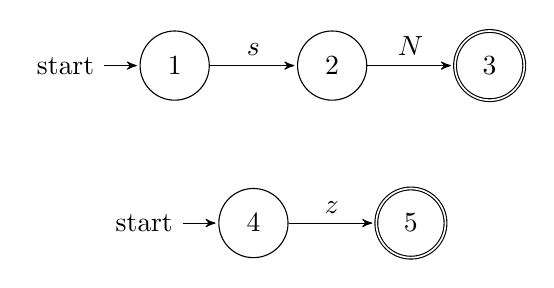
\begin{tikzpicture}[->,>=stealth',shorten >=1pt,auto,node distance=2cm,
    scale = 1,transform shape]

  \node[state,initial] (1) {$1$};
  \node[state] (2) [right of=1] {$2$};
  \node[state,accepting] (3) [right of=2] {$3$};
  \node[state,initial] (4) [below of=1, xshift=1cm] {$4$};
  \node[state,accepting] (5) [right of=4] {$5$};

  \path (1) edge              node {$s$} (2)
  (2) edge              node {$N$} (3)
  (4) edge              node {$z$} (5);

\end{tikzpicture}
\end{center}

We then combine them into a single pushdown automata by replacing each edge with a non-terminal label $p \xrightarrow{N} q$ with ($+\gamma$ means ''push $\gamma$'', while $-\gamma$ means ''pop $\gamma$''):

\begin{itemize}
  \item An edge $p \xrightarrow{'(', +(p, q)} p'$ for every initial state $p'$ in some DFA belonging to non-terminal $N$.
  \item An edge $q' \xrightarrow{')', -(p, q)} q$ for every final state $q'$ in some DFA belonging to non-terminal $N$.
\end{itemize}

\begin{center}
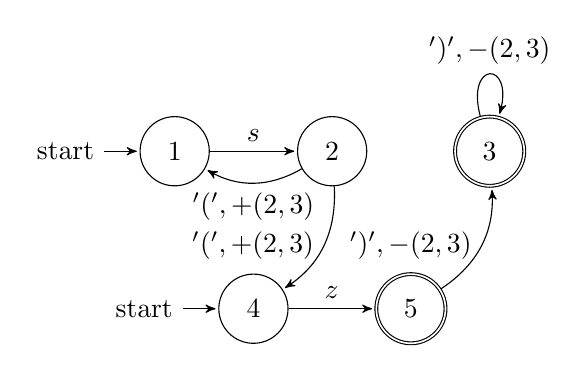
\begin{tikzpicture}[->,>=stealth',shorten >=1pt,auto,node distance=2cm,
    scale = 1,transform shape]

  \node[state,initial] (1) {$1$};
  \node[state] (2) [right of=1] {$2$};
  \node[state,accepting] (3) [right of=2] {$3$};
  \node[state,initial] (4) [below of=1, xshift=1cm] {$4$};
  \node[state,accepting] (5) [right of=4] {$5$};

  \draw
  (1) edge[above] node{$s$} (2)
  (4) edge[above] node{$z$} (5)
  (2) edge[bend left, below] node{$'(', +(2, 3)$} (1)
  (2) edge[bend left, left] node{$'(', +(2, 3)$} (4)
  (3) edge[loop above] node{$')', -(2, 3)$} (3)
  (5) edge[left, bend right] node{$')', -(2, 3)$} (3);

\end{tikzpicture}
\end{center}

\noindent Finally, we add a new initial state and a new final state, and connect them with the initial and final states belonging to the starting non-terminal:

\begin{center}
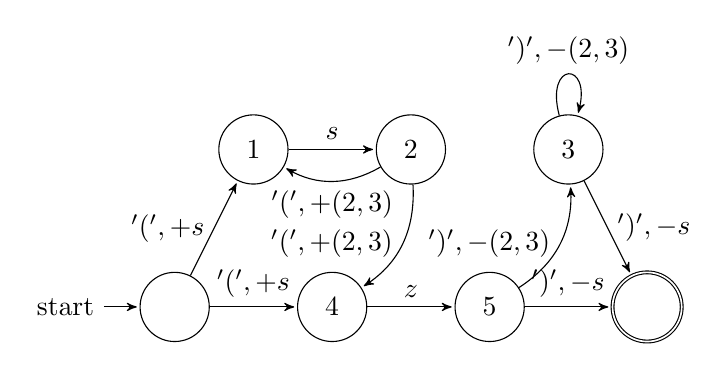
\begin{tikzpicture}[->,>=stealth',shorten >=1pt,auto,node distance=2cm,
    scale = 1,transform shape]

  \node[state] (1) {$1$};
  \node[state] (2) [right of=1] {$2$};
  \node[state] (3) [right of=2] {$3$};
  \node[state] (4) [below of=1, xshift=1cm] {$4$};
  \node[state] (5) [right of=4] {$5$};
  \node[state,initial] (s) [left of=4] {};
  \node[state,accepting] (e) [right of=5] {};

  \draw
  (s) edge[left] node{$'(', +s$} (1)
  (s) edge[above] node{$'(', +s$} (4)
  (3) edge[right] node{$')', -s$} (e)
  (5) edge[above] node{$')', -s$} (e)
  (1) edge[above] node{$s$} (2)
  (4) edge[above] node{$z$} (5)
  (2) edge[bend left, below] node{$'(', +(2, 3)$} (1)
  (2) edge[bend left, left] node{$'(', +(2, 3)$} (4)
  (3) edge[loop above] node{$')', -(2, 3)$} (3)
  (5) edge[left, bend right] node{$')', -(2, 3)$} (3);

\end{tikzpicture}
\end{center}

\noindent The resulting pushdown automaton has only a single source of non-determinism: the edges labelled \verb|'('|. Each one corresponds to one of the allowable child productions at that point in the parse tree.

%% \noindent Generalizing this to a complete grammar, we get the following property: a grammar $G$ is resolvable iff:

%% $$
%% \begin{array}{l}
%%   \forall t \in L(T).\\
%%   \quad \exists w' \in L(G').\\
%%   \qquad \forall t' \in L(T').\ \yield(t') = w' -> \unparen(t') = t
%% \end{array}
%% $$


%%%%%%%%%%%%%%%%%%%%%%%%%%%%%%%%%%%%%%%%%%%%%%%%%%%%%%%%%%%

%% \begin{theorem}
%%   If $\{(, )\} \cap \T = \emptyset$, then any unambiguous word $w \in L(G)$ is resolvable.
%% \end{theorem}

%% \noindent \textbf{Proof.} Since $w$ is unambiguous in $G$ there is exactly one parse tree $t \in L(T)$ such that $\yield(t) = w$. Since $L(G) \subseteq L(G')$ we have that $w \in L(G')$. Furthermore, $w$ is unambiguous in $L(G')$ as well, since no added productions can apply (they all contain parentheses, which cannot be present in $w$). Additionally, since $L(T) \subseteq L(T')$, we have that $t \in L(T')$, and since $\yield(t) = w$, it must be the only parse tree for $w$ in $L(T')$. Finally, $\unparen(t) = t$.

%%%%%%%%%%%%%%%%%%%%%%%%%%%%%%%%%%%%%%%%%%%%%%%%%%%%%%%%%%%

%% %% Acknowledgments
%% \begin{acks}                            %% acks environment is optional
%%                                         %% contents suppressed with 'anonymous'
%%   %% Commands \grantsponsor{<sponsorID>}{<name>}{<url>} and
%%   %% \grantnum[<url>]{<sponsorID>}{<number>} should be used to
%%   %% acknowledge financial support and will be used by metadata
%%   %% extraction tools.
%%   This material is based upon work supported by the
%%   \grantsponsor{GS100000001}{National Science
%%     Foundation}{http://dx.doi.org/10.13039/100000001} under Grant
%%   No.~\grantnum{GS100000001}{nnnnnnn} and Grant
%%   No.~\grantnum{GS100000001}{mmmmmmm}.  Any opinions, findings, and
%%   conclusions or recommendations expressed in this material are those
%%   of the author and do not necessarily reflect the views of the
%%   National Science Foundation.
%% \end{acks}


%% Bibliography
\bibliography{All}


%% %% Appendix
%% \appendix
%% \section{Appendix}

%% Text of appendix \ldots

\end{document}
